%\subsection{Heat Pump}
\subsubsection{Heat Pump}

A heat pump can be modeled in several ways. A straightforward approach is to reduce the heat pump to two \textsf{FixedNode} objects, external to the building system. These nodes represent the evaporator and condensor \emph{exit} temperatures $T_{evap}$ and $T_{cond}$. In case of a air-water heatpump, $T_{evap}$ can be approximated with the instantaneous outdoor (ambient) temperature from the weather conditions. For a heat pump with a liquid heat source this will be the source temperature, in any cases a ground source. $T_{cond}$ can be derived from a heating curve ($T_{cond}$ vs. $T_{outdoor}$) or from a heat pump functional model.

The elements of the heat pump model are:

\begin{itemize}
	\item a "hot" condensor node $T_{cond}$. This is a node of type \textsf{FixedNode} or \textsf{CapacityNode}(see section \ref{sec:capnode}).
	\item a "cold" condensor node $T_{return}$. This is a node of type \textsf{FixedNode} (see section \ref{sec:fixnode}), with a variable temperature, but no heat capacity.
	\item an "ambient" temperature $T_{evap}$ at the evaporator side of the heat pump \textit{i.e.} the "outdoor" node of the building in the model.
	\item a \textsf{Flow} object with a \textsf{node\_list} starting at the hot node, passing through \textit{e.g.} a buffer vessel. There, (part of) the thermal energy is stored. Via the bottom layer of the vessel the flow returns to the cold condensor node.  Thermal power is added by the heat pump, to increase the temperature of the water from $T_{return}$ to $T_{cond}$. The flow object has an attribute $F_{hp}$ which equals the magnitude of the thermal heat transfer in $[W/K]$.
	\item the instantaneous thermal power $\dot{q}_{hp}$, delivered by the heat pump to the condensor flow circuit and the buffer vessel. Equals $F_{hp} \cdot (T_{cond} - T_{return})$. The maximal value of $\dot{q}_{hp}$ is a function of of $T_{cond}$ and $T_{evap}$.
	\item the instantaneous electric power $P_{el}$. Usually, a heat pump has characteristic curves, giving the \emph{coefficient of performance (COP)} as a function of $T_{cond}$ and $T_{evap}$. COP equals $\dot{q}_{hp}/P_{el}$. 
\end{itemize} 

\begin{figure}[h!]
	\begin{center}
		\begin{circuitikz}
			\ctikzset{bipoles/thickness=3}
			\draw (8,0)
			node[color=darkgreen, circ, label={[darkgreen]above:$T_{bottom}$}]{}
			to[R,R=$R_{mid,bot}$] (8,4) 
			node[color=darkgreen, circ, label={[darkgreen]above:$T_{mid}$}]{}
			to[R,R=$R_{top,mid}$, -*] (8,8)
			node[color=darkgreen, circ, label={[darkgreen]above:$T_{top}$}]{};
			\draw (8,0)
			node[color=darkgreen, circ, label={[darkgreen]above:$T_{bottom}$}]{}
			to[R,R=$R_{mid,bot}$] (8,4) 
			node[color=darkgreen, circ, label={[darkgreen]above:$T_{mid}$}]{}
			to[R,R=$R_{top,mid}$, -*] (8,8)
			node[color=darkgreen, circ, label={[darkgreen]above:$T_{top}$}]{};
			\draw (8.5,0)
			to [short] (8.5,8)
			to [short] (11,8)
			to [short] (11,5)
			to [short] (12,5)
			node[color=red, circ, label={[red]above:$T_{feed}$}]{}
			to [short, *-*] (12,3)
			node[color=blue, circ, label={[blue]above:$T_{return}$}]{}
			to [short] (11,3)
			to [short] (11,0)
			to [short] (8.5,0)
			(16,4) to[amp, label=$\dot{Q}_{heat pump}$] ++(-4,0);
		\end{circuitikz}
		\caption{Heat pump model.}
		\label{fig:hpmodel}
	\end{center}
\end{figure}

In Fig.~\ref{fig:hpmodel} a heat pump is shown with its nodes, surroundings and a buffer vessel for generating a supply and return flow. The heat pump will deliver its thermal power via an internal heat exchanger from the condensor side to a liquid heat carrier (water) in a buffer vessel. For the liquid medium, the following equation holds:

\begin{equation}\color{blue}
	\label{eq:hpflow}
	\begin{aligned}
		F_{hp} &= \dot{f} \cdot \rho \cdot c_w  &= \dot{m} \cdot c_w 
	\end{aligned}
\end{equation}

where: \\
$\rho$ is the density of the medium in $[kg/m^3]$ \\
$c_w$ is the specific heat capacity of water: $4.2 \cdot 10^3 J/(kg \cdot K)$ \\
$\dot{f}$ is the liquid volume flow in $[m^3/s]$ \\
$\dot{m}$ is the liquid mass flow in $[kg/s]$ \\

There are a few options for the connection of the buffer vessel:

\subsubsection{4-way connection}

The most straightforward connection method is a 4-way connection, as shown in Figure~\ref{fig:4way}. The heat source (heat pump) thermally loads the buffer vessel in the top layer. The thermal demand is also taken from the top layer. For low-temperature radiators or a floor heating circuit there is a mixing valve that short circuits feed and return water, to provide an adjustable temperature heat source for the delivery system. The remaining return flow from the delivery system is passed back to the bottom layer of the buffer vessel. The heat source return water is also taken from the bottom layer.

\begin{figure}[H]
	\centering
	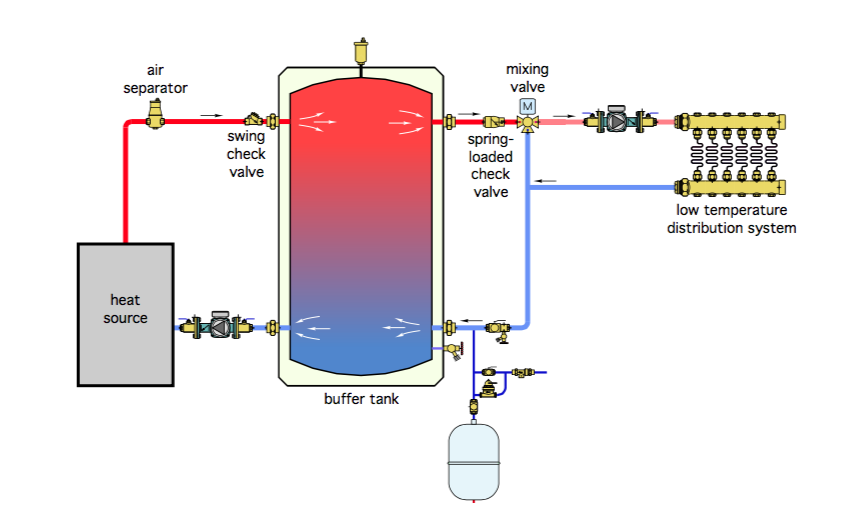
\includegraphics[width=0.7\columnwidth]{Figures/4-way buffer connection}
	\caption[Short title]{4-way connection of stratified buffer vessel.}
	\label{fig:4way}
\end{figure} 

\begin{figure}[H]
	\centering
	\begin{subfigure}[b]{0.45\textwidth}
		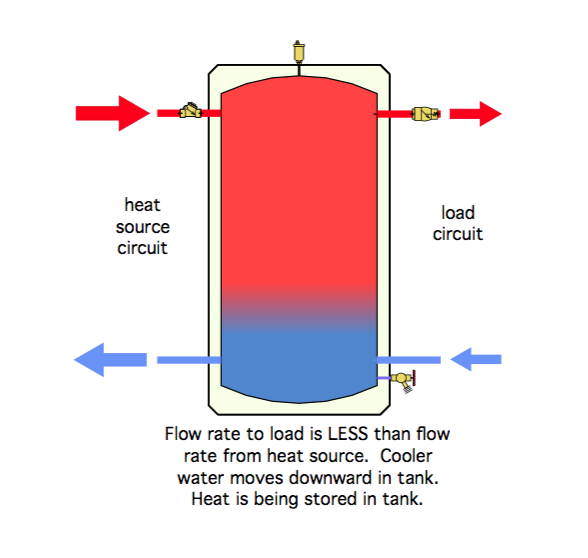
\includegraphics[width=\textwidth]{Figures/4-way buffer loaded}
		\caption{Buffer vessel loading...}
		\label{fig:4way_loaded}
	\end{subfigure}
	\hfill
	\begin{subfigure}[b]{0.45\textwidth}
		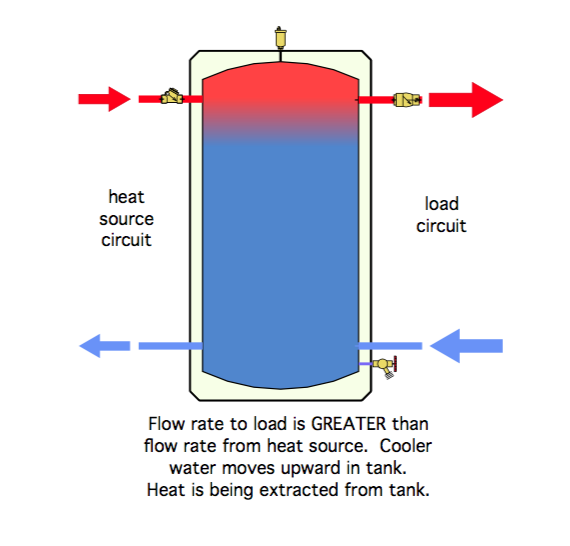
\includegraphics[width=\textwidth]{Figures/4-way buffer unloading}
		\caption{Buffer vessel unloading...}
		\label{fig:4way_unloading}
	\end{subfigure}
	\caption{Stratified buffer vessel dynamics.}
	\label{fig:4way_dynamics}
\end{figure}

\subsubsection{2-way connection}

\begin{figure}[H]
	\centering
	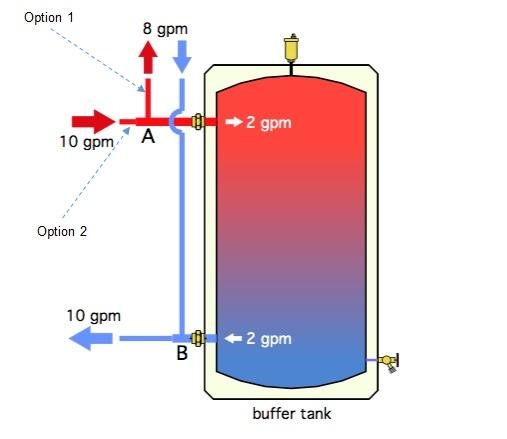
\includegraphics[width=0.5\columnwidth]{Figures/2-way buffer connection}
	\caption[Short title]{2-way connection of stratified buffer vessel.}
	\label{fig:2way}
\end{figure} 


The \textsf{HeatPump} class in Python encapsulates the attributes above and the calculation of $F_{hp}$. The methods of this class are:
\begin{itemize}
	\item \textsf{\_\_init\_\_}: initializes the class members. Members starting with \_\_* are private members.
\end{itemize}

\lstinputlisting[label=lst:Radiator, linerange={102-151}, 
caption={HeatPump class}] 
{../../housemodel/sourcesink/radiators/radiators.py}

\begin{itemize}
	\item \textsf{from\_dict}. This method operates as an "overloaded" constructor, reading from a Python \textsf{dictionary}.
\end{itemize}

\lstinputlisting[label=lst:Radiator, linerange={153-157}, 
caption={Radiator class}] 
{../../housemodel/sourcesink/radiators/radiators.py}

\begin{itemize}
	\item \textsf{get\_gmtd} and \textsf{get\_lmtd}: return the value of private member \_\_gmtd or \_\_lmtd.
\end{itemize}

\lstinputlisting[label=lst:Radiator, linerange={175-179}, 
caption={Radiator class}] 
{../../housemodel/sourcesink/radiators/radiators.py}

The Radiator class uses helper functions \textsf{GMTD\_radiator} and \textsf{LMTD\_radiator} to determine the effective temperature difference from $T_{supply}$, $T_{return}$ and $T_{indoor}$:

\lstinputlisting[label=lst:lmtd, linerange={22-70}, 
caption={GMTD\_radiator and LMTD\_radiator helper functions}] 
{../../housemodel/sourcesink/radiators/radiators.py}

In the building model, a fluid flow through the radiator leads to the delivery of heat to the room(s). The equations for the heat transfer of the radiator are: 

{\color{blue}
	\begin{equation}
		\label{eq:radnonlin}
		\begin{aligned}
			\dot{q}_{rad} &- K_m \cdot (\Delta T_{LMTD})^n &= 0 \\
			\dot{q}_{rad} &- F_{rad} \cdot (T_{feed} - T_{return}) &= 0 \\ \\
			&\text{with } \Delta T_{LMTD} = \frac{T_{feed} - T_{return}}{\ln\left(\frac{T_{feed} -T_{air}}{T_{return} - T_{air}}\right)}
		\end{aligned}
	\end{equation}
}

In the building model, this nonlinear system of equations can be solved for the two unknowns $[\dot{q}_{rad} \quad T_{return}]$, if input data $T_{supply}$, $ T_{ind}$, $C_{rad}$ and $F_{rad}$ are provided. A solver for such a system of equations needs the function template in Eq.~\ref{eq:radnonlin}, with the unknowns vector as input variable. Furthermore, the Jacobian of the function template has to be calculated. Evaluation of an analytical expression of the partial derivatives in the Jacobian always outperforms numerical derivative calculations. Thus, for the upper equation (function) in set \ref{eq:radnonlin}:

\begin{equation}
	\begin{aligned}
		\begin{matrix}
			\frac{\partial f}{\partial \dot{Q}_{rad}} &= 1 \\ 
			\\
			\dfrac{\partial f}{\partial T_{return}} &= -Cn\cdot \dfrac{\left(\frac{T_1-T_2}{\ln\left(\frac{T_1-T_3}{T_2-T_3}\right)}\right)^{n-1}\,\left(\frac{T_1-T_2}{T_2-T_3}-\ln\left(\frac{T_1-T_3}{T_2-T_3}\right)\right)}{\ln^2\left(\frac{T_1-T_3}{T_2-T_3}\right)} \\ \\
		\end{matrix}
	\end{aligned}
\end{equation} 
for the second equation:
\begin{equation}
	\begin{aligned}
		\begin{matrix}
			\frac{\partial f}{\partial \dot{Q}_{rad}} &= 1 \\ \\
			\frac{\partial f}{\partial T_{return}} &= F_{rad}
		\end{matrix}
	\end{aligned}
\end{equation} 

See: \url{https://www.derivative-calculator.net/}.

The Jacobian matrix becomes:
\begin{equation}
	\begin{aligned}
		\mathbf{J}_{i,j}=\dfrac{\partial f_{i}(\mathbf{x})}{\partial x_{j}} =
		\begin{bmatrix}
			\dfrac{\partial f_1}{\partial \dot{Q}_{rad}} & \dfrac{\partial f_1}{\partial T_{return}} \\ 
			\vspace{2pt} \\
			\dfrac{\partial f_2}{\partial \dot{Q}_{rad}} & \dfrac{\partial f_2}{\partial T_{return}}
		\end{bmatrix}
		\qquad
		\mathbf{x} =
		\begin{bmatrix}
			\dot{q}_{rad} \\ 
			T_{return}
		\end{bmatrix}
	\end{aligned}
\end{equation} 

As an alternative, $\Delta T_{GMTD})$ can be used. The set of equations becomes:

{\color{blue}
	\begin{equation}
		\label{eq:radgmtd}
		\begin{aligned}
			\dot{q}_{rad} &- K_m \cdot (\Delta T_{GMTD})^n &= 0 \\
			\dot{q}_{rad} &- F_{rad} \cdot (T_{s} - T_{r}) &= 0 \\ \\
			&\text{with } \Delta T_{GMTD} = \sqrt{\Delta T_{s,ind}} \cdot  \sqrt{(T_{return} - T_{ind}})
		\end{aligned}
	\end{equation}
}

Note the left-hand side of the first equation can be written as:
$$ \dot{q}_{rad} - K_{m} \cdot \left(\Delta T_{s,ind}\right)^{n/2} \cdot \left(T_{return} - T_{ind}\right)^{n/2} $$

Thus, for the upper equation (function) in set \ref{eq:radgmtd}:

\begin{equation}
	\begin{aligned}
		\begin{matrix}
			\dfrac{\partial f}{\partial T_{return}} &= - K_{m} \cdot \left(\Delta T_{s,ind}\right)^{n/2} \cdot \dfrac{n}{2} \cdot \left(T_{return} - T_{ind}\right)^{(n/2)-1} \\ \\
		\end{matrix}
	\end{aligned}
\end{equation} 

The calculations for solving the vector $\mathbf{x} = [\dot{q}_{rad} \quad T_{return}]^T$ are performed in the method \textsf{update}. This method uses the Newton-Rhapson algorithm in \textsf{scipy.optimize.root()} to find the roots $\mathbf{x}$ of the radiator equations.
The input argument for the \textsf{scipy.optimize.root()} method can be \textsf{func\_rad\_gmtd} or \textsf{func\_rad\_lmtd}. These functions calculate the radiator equations and their partial derivatives in the Jacobian.

\lstinputlisting[label=lst:lmtd, linerange={181-230}, 
caption={\textsf{func\_rad\_gmtd} and \textsf{func\_rad\_lmtd} function templates for \textsf{scipy.optimize.root()}}] 
{../../housemodel/sourcesink/radiators/radiators.py}

\lstinputlisting[label=lst:lmtd, linerange={232-241}, 
caption={\textsf{update} method caaling \textsf{scipy.optimize.root()}}]
{../../housemodel/sourcesink/radiators/radiators.py}

A discussion about the underlying radiator models can be found in \cite{TolRadiator, TolThesis}. The radiator equations use the (normative) guidelines in \cite{NEN442}. See also Appendix~\ref{app::radeq}.

In the radiator model, there is a choice for the data type of the node with $T_{supply}$, and a (virtual) node with temperature $T_{indoor} + \Delta T$. In the simplest version of the radiator model, these nodes are of type \textsf{FixedNode}. A consequence is, that the radiator has no heat capacity. Moreover, once the demand flow stops, the heat input to the building interior stops instantaneously. If water flows through the radiator, the $\mathbf{DF_{demand}}$-matrix of the demand flow will remain symmetric, but will get extra contributions to the diagonal elements. It may be a good idea to split the $\mathbf{F}$-matrix into two parts, $\mathbf{F_{int}}$ and $\mathbf{F_{ext}}$. Thus, the thermal flow \emph{between} the \textsf{CapacityNodes} and from the \textsf{FixedNodes} to the \textsf{CapacityNodes} can be separately calculated. In the current (simplest) version, $\mathbf{F_{int}}$ contains no entries from the radiator. All contributions are on the diagonal of the $\mathbf{F_{ext}}$ and on the corresponding row of the $\dot{q_{F}}$-vector.

\newpage
